
% VLDB template version of 2020-08-03 enhances the ACM template, version 1.7.0:
% https://www.acm.org/publications/proceedings-template
% The ACM Latex guide provides further information about the ACM template


\documentclass[sigconf, nonacm]{acmart}

\usepackage{array}
\usepackage{catchfile}
%% The following content must be adapted for the final version
% leave empty if no availability url should be set
\newcommand\vldbavailabilityurl{https://doi.org/10.5281/zenodo.10711084}

\begin{document}
\title{Evaluating Performance of YFilter's Approach to Nested Path Expression Processing}

%%
%% The "author" command and its associated commands are used to define the authors and their affiliations.
\author{Emily Courtney}
\affiliation{%
  \institution{University of Passau}
  \city{Passau}
  \country{Germany}
}
\email{emily.courtney@uni-passau.de}

\maketitle

%%% do not modify the following VLDB block %%
%%% VLDB block start %%%
\ifdefempty{\vldbavailabilityurl}{}{
\vspace{.3cm}
\begingroup\small\noindent\raggedright\textbf{PVLDB Artifact Availability:}\\
The source code, data, and/or other artifacts have been made available at \url{\vldbavailabilityurl}.
\endgroup
}
%%% VLDB block end %%%

\section{Introduction}

YFilter \cite{yfilter} is an XML filtering system that aims to provide fast, on-the-fly matching of XML encoded data to a large number of queries. The development of YFilter builds off insights from the XFilter system~\cite{xfilter}, which was the first published Finite State Machine-based XML filtering approach. YFilter uses a different approach, and combines all of the path queries into a single Nondeterministic Finite Automaton. It exploits similarities of queries by merging common prefixes of the query paths so that they are processed at most once, resulting in significant improvements in structure matching performance.~\cite{yfilter}

In the article ``Path Sharing and Predicate Evaluation
for High-Performance XML Filtering,''~\cite{yfilter} both the XFilter and YFilter approaches are described in detail, and experiments are performed to compare the two approaches. Next, two alternative techniques for handling value-based predicates are proposed, and their performance is evaluated. Finally, a description of how the YFilter approach handles more complicated queries containing nested path expressions is given, and an evaluation of this approach is described.

The source code for YFilter can be found online~\cite{yfilter_source}. However, the implementation of the XFilter algorithm used in the study is not available. And while the pseudo-code for the alternate predicate-handling techniques is given in the paper, the implementation is also not available. There is one experiment which only requires the standard YFilter software, so that is the experiment looked at in this report. 

While the same source code~\cite{yfilter_source} used in the original study is available, not all of the data artifacts are available, and so we consider this to be a replication as opposed to a reproduction. 

\section{Experiment Details}

The experiment being replicated here is an evaluation of the performance of YFilter's approach to processing nested path expressions. In the experiment, YFilter is run repeatedly with different sets of queries. The query sets vary in the number of distinct queries and the number of nested path expressions in each query.

The performance metric used is called ``multiquery processing time (MQPT),'' which captures all costs attributable to the filtering algorithms themselves~\cite{yfilter}. MQPT is calculated as the filtering time minus the document parsing time, which are both output when the YFilter program runs.

\begin{figure}
  \centering
  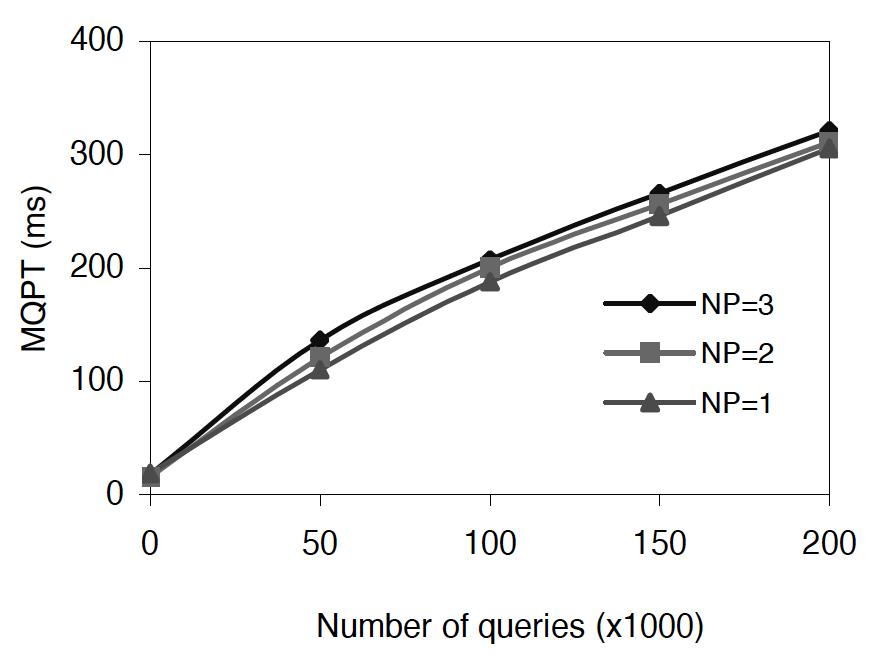
\includegraphics[width=0.75\linewidth]{results/reference_figure.png}
  \caption{Results from original study~\cite{yfilter}}
  \label{fig:reference_figure}
\end{figure}

In the original study, a trend was observed from Figure \ref{fig:reference_figure}. As the number of queries grows, MQPT increases to process the first nested path queries. However, processing additional nested paths costs only a little more than processing the first nested paths.~\cite{yfilter}

As this figure is the only thing from the experiment results available to us, we will compare the results of our replication to this graph. We consider our replication experiment to be successful if we observe the same trend on our graph. Specifically, we look for the following:

\begin{enumerate}
    \item There is an increase in MQPT for each successive increase in number of queries processed.

    \item For each number of queries being processed, the cases of larger NP values exhibit efficiency and scalability very close to that in the case of NP=1~\cite{yfilter}.
\end{enumerate}


\section{Replication Setup}

To run the experiment, we require the YFilter program, a set of XML documents, and a set of queries. 

The YFilter program was downloaded from the project website~\cite{yfilter_source}. The resources include both the source code and pre-compiled executables of the program. Since our replication is using the original program without any modifications, we decided to use the given executables rather than compiling them ourselves. 

The original study used a set of 200 XML documents, generated using IBM's XML Generator~\cite{IBM_XML}. While the XML documents used in the study are not available, the YFilter project does include a set of XML documents that the original team generated with the same settings. So, in our replication, we choose 200 of these documents. To make it more clear where to find the data in our reproduction package, we copied the XML documents from the YFilter package into our own \texttt{data/xml} directory of both the github repository and the docker container.

The set of queries used in the original study is also not available. However, a query generator is included in the YFilter project, and the workload settings used to generate the query sets are described in detail. So, for our replication, we use the provided query generator and the stated workload settings to produce query sets.

Since the query generator does not produce static results, we also decided to generate the queries ahead of time, and to copy them directly into the docker container. This enables us to use the same set of query documents when repeating the experiment. The generated query files, along with the script used to generated them, can be found in the \texttt{data/queries} directory.

When generating queries, the parameter NP is used to generate a number of nested path expressions in each query~\cite{yfilter}. The original experiment evaluates the performance of YFilter as the number of distinct queries is varied from 1000 to 200,000, with NP equal to 1, 2, and 3. For our experiment, we use the same values for NP and the same range of queries.

Finally, in the original study, the Java Virtual Machine is run with a maximum allocation pool of 250MB, so that virtual memory and other I/O-activity did not influence the results~\cite{yfilter}. We do the same in our experiment.

\section{Replication Results}

\begin{figure}
  \centering
  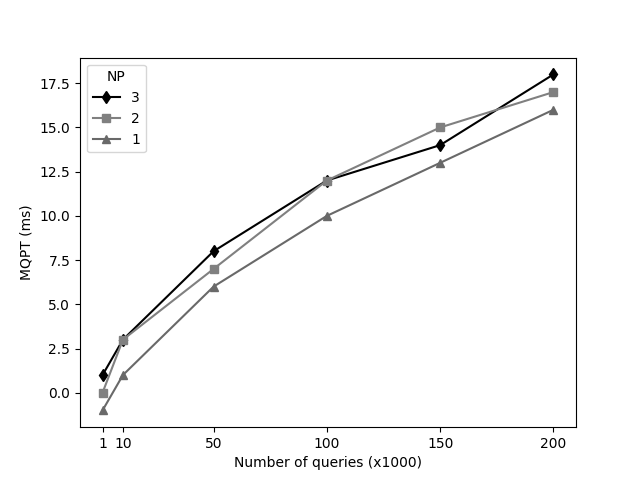
\includegraphics[width=\linewidth]{results/replication_figure.png}
  \caption{Results from the replicated experiment}
  \label{fig:replication_figure}
\end{figure}

\begin{table}
  \begin{center}
  \caption{MQPT values from the replicated experiment}

\label{table:results_table}

\CatchFileDef{\resultstable}{results/results_table.tex}{}
\begin{tabular}{r r r r}\toprule
  \textbf{NP} & \textbf{1} & \textbf{2} & \textbf{3} \\\midrule
  \textbf{Queries} & & & \\\midrule
  \resultstable
  \bottomrule
\end{tabular}

  \end{center}
\end{table}


The results of the replicated experiment can be seen in Figure \ref{fig:replication_figure} and in Table \ref{table:results_table}.

One of the first things to notice is that the processing time is significantly less than in the original experiment. Instead of dealing with processing times in the range of 100-400ms, we instead see a range of about 0-25ms. The increased processing power of our machine is one potential threat to validity, but, since we are evaluating the relative difference of processing time for additional nested path expressions, this does not pose a problem for our replication.

We also noticed that the processing time for 1000 queries is so small that it is not accurately measured in milliseconds. This is another potential threat to validity, and so we decided to add an additional query set of 10,000 queries to better distinguish the lower-end of processing time.

When considering whether or not this is a successful replication, the first trend we expect to see is that there is an increase in MQPT for each successive increase in number of queries processed. Looking at our results, we can see that this trend is present.

Next, we want to see that the cases of larger NP values exhibit efficiency and scalability very close to that in the case of NP=1.
This criterion takes a bit more consideration. It is interesting to see that, unlike in the original experiment, we actually observe smaller MQPT values for higher number of nested path expressions in some cases. We believe this is a result of the faster processing times. Here it is helpful to look at Table \ref{table:results_table}. We can see that the range of processing times for each number of queries is within about 3ms, and so there is not much variation in the time needed to process different number of nested path expressions. Because of this, we consider the second trend to also be present.

Therefore, since we see both of the required criteria in our data, we consider this to be a successful replication of the original experiment.

\bibliographystyle{ACM-Reference-Format}
\bibliography{references}

\end{document}
\endinput
